% \iffalse
\let\negmedspace\undefined
\let\negthickspace\undefined
\documentclass[journal,12pt,onecolumn]{IEEEtran}
\usepackage{cite}
\usepackage{amsmath,amssymb,amsfonts,amsthm}
\usepackage{algorithmic}
\usepackage{graphicx}
\usepackage{textcomp}
\usepackage{xcolor}
\usepackage{txfonts}
\usepackage{listings}
\usepackage{enumitem}
\usepackage{mathtools}
\usepackage{gensymb}
\usepackage{comment}
\usepackage[breaklinks=true]{hyperref}
\usepackage{tkz-euclide} 
\usepackage{listings}
\usepackage{gvv}                                        
\def\inputGnumericTable{}                                 
\usepackage[latin1]{inputenc}                                
\usepackage{color}                                            
\usepackage{array}                                            
\usepackage{longtable}                                       
\usepackage{calc}                                             
\usepackage{multirow}                                         
\usepackage{hhline}                                           
\usepackage{ifthen}                                           
\usepackage{lscape}

\newtheorem{theorem}{Theorem}[section]
\newtheorem{problem}{Problem}
\newtheorem{proposition}{Proposition}[section]
\newtheorem{lemma}{Lemma}[section]
\newtheorem{corollary}[theorem]{Corollary}
\newtheorem{example}{Example}[section]
\newtheorem{definition}[problem]{Definition}
\newcommand{\BEQA}{\begin{eqnarray}}
\newcommand{\EEQA}{\end{eqnarray}}
\newcommand{\define}{\stackrel{\triangle}{=}}
\theoremstyle{remark}
\newtheorem{rem}{Remark}
\begin{document}
\bibliographystyle{IEEEtran}
\vspace{3cm}

\title{NCERT-discrete : 11.9.3 - 21}
\author{EE23BTECH11025 - Anantha Krishnan $^{}$% <-this % stops a space
}
\maketitle
\bigskip

\renewcommand{\thefigure}{\theenumi}
\renewcommand{\thetable}{\theenumi}
\section{question}
Find four numbers forming a geometric progression in which the third term is greater than the first term by 9, and the second term is greater than the $4^{th}$ by 18.\\

\textbf{Solution}:
\vspace{0.5cm}
\begin{enumerate}
\begin{tabular}{ |c|c|c| } 
 \hline
Symbols & Description & Values  \\
\hline
 $r$ & Common ratio of the GP & -2\\
 \hline

  $x(n)$ & $(n+1)^{th}$ term of the Sequence & \ $x(0)r^{n}u(n)$\\
  \hline


  $x(0)$ & First term of the GP & 3\\
\hline
  
   \hline
\end{tabular}
\end{enumerate}
\centering
\captionsetup{Table 1 : Parameters , Descriptions And Values }
\label{table:ee25-tab2}
\vspace{0.5cm}

\begin{enumerate}
    \item Solving for $x(0)$,$x(1)$,$x(2)$,$x(3)$ :
   \begin{align}
x(0)r^2 - 9 &= x(0) \label{eq:ee25-a1}\\
x(0)r + 18 &= x(0)r^3\label{eq:ee25-a2}
\end{align}
Solving  \eqref{eq:ee25-a1} , \eqref{eq:ee25-a2}
\begin{align}
    x(0) &= 3\\
    r &= -2
\end{align}
Therefore 
\begin{align}
    x(0) &= 3\\
    x(1) &= -6\\
    x(2) &= 12\\
    x(3) &= -24
     \end{align}

    \item Z-Transform for x(n) 
    Using $\eqref{eq:ztrans}$ :
    \begin{align}
    X(z) &= \sum_{n=-\infty}^{\infty}(3(-2)^nu(n))z^{-n} \\
    &= z(2+z)^{-1} ,\quad \abs {z}>\abs{2} 
    \end{align}
    
\end{enumerate}
    \begin{figure}[!ht]
    \centering
\graphicspath{ {figs/} }
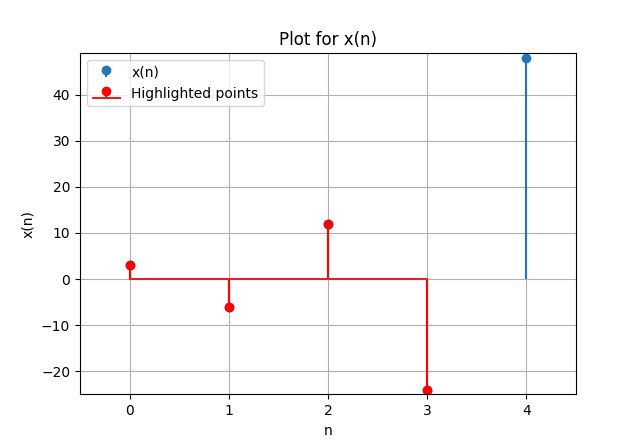
\includegraphics[width=12cm, height=8cm]{graph_1}
\caption{ $x(n)$ vs n }
\label{graph:ee25-ag2}
\end{figure}
\vspace{0.5cm}







 






\end{document}
